\section{数列极限的基本性质}\label{sec:1.2}

在定义了数列极限之后，我们会用 $\varepsilon\text{-}N$ 法证明一些数列的极限，但从上节知道，这必须在已知数列有无极限的前提下才能应用，且某些证明还相当复杂，有些甚至还无法用 $\varepsilon\text{-}N$ 法证明。所以，我们必须进一步了解数列极限有哪些性质，还有什么方法可以使用。为此，本节将逐一给出数列极限的唯一性，收敛数列的有界性，极限的四则运算性质，不等式性质以及重要的夹逼定理。

\begin{theorem}[极限的惟一性]\label{thm:1.2.1}
设数列 $\{a_{n}\}$ 有极限（实数，或 $+\infty$，或 $-\infty$），则极限是惟一的。
\end{theorem}

\begin{proof}
\textbf{证法 1} 设 $\lim\limits_{n\to+\infty}a_n=a$ 及 $\lim\limits_{n\to+\infty}a_n=b$，$a,b\in\mathbb{R}$。

（反证）反设 $a \neq b$。令 $\varepsilon_{0} = |a - b| > 0$，根据数列极限的定义~\ref{def:1.1.1}，$\exists N \in \mathbb{N}$，当 $n > N$ 时，
\[
|a_{n}-a|<\frac{\varepsilon_{0}}{2},\quad |a_{n}-b|<\frac{\varepsilon_{0}}{2},
\]
所以，
\[
|a-b| \leqslant |a-a_{n}| + |a_{n}-b| < \frac{\varepsilon_{0}}{2} + \frac{\varepsilon_{0}}{2} = \varepsilon_{0} = |a-b|,
\]
矛盾。

值得注意的是这种证法不能应用到极限为 $+\infty$ 或 $-\infty$ 的情况，因此还必须给出能推广到 $+\infty$ 或 $-\infty$ 的证法，于是有下面证法。

\textbf{证法 2} 设 $\lim\limits_{n\to+\infty}a_n=a$ 及 $\lim\limits_{n\to+\infty}a_n=b$，$a,b\in\mathbb{R}$。

（反证）反设 $a \neq b$，不失一般性，设 $a < b$。令 $\varepsilon_{0} = \frac{b - a}{2} > 0$。由极限定义~\ref{def:1.1.1} 知，$\exists N_{1} \in \mathbb{N}$，当 $n > N_{1}$ 时，$a - \varepsilon_{0} < a_{n} < a + \varepsilon_{0}$；$\exists N_{2} \in \mathbb{N}$，当 $n > N_{2}$ 时，$b - \varepsilon_{0} < a_{n} < b + \varepsilon_{0}$。所以，当 $n > N = \max\{N_{1}, N_{2}\}$ 时，
\[
\frac{a+b}{2} = b - \frac{b-a}{2} = b - \varepsilon_{0} < a + \varepsilon_{0} = a + \frac{b-a}{2} = \frac{a+b}{2},
\]
矛盾。

其他情形类似证明。

\textbf{证法 3}（统一描述）设 $\lim\limits_{n\to+\infty}a_n=a$ 及 $\lim\limits_{n\to+\infty}a_n=b$。

（反证）反设 $a \neq b$，不妨设 $a < b$，则存在 $a$ 的开邻域 $U_a$ 与 $b$ 的开邻域 $U_b$，使得 $U_a \cap U_b = \varnothing$。由极限定义~\ref{def:1.1.1} 知，$\exists N_1 \in \mathbb{N}$，当 $n > N_1$ 时，$a_n \in U_a$；$\exists N_2 \in \mathbb{N}$，当 $n > N_2$ 时，$a_n \in U_b$。所以，当 $n > \max\{N_1, N_2\}$ 时，$a_n \in U_a \cap U_b = \varnothing$，矛盾。
\end{proof}

\begin{definition}\label{def:1.2.1}
如果存在实数 $M>0$，使得对任何自然数 $n$，有 $|a_{n}| \leqslant M$，则称数列 $\{a_{n}\}$ \textbf{有界}。如果存在实数 $B$，使得 $a_{n} \leqslant B$（$\forall n \in \mathbb{N}$），则称数列 $\{a_{n}\}$ \textbf{有上界} $B$。如果存在实数 $A$，使得 $a_{n} \geqslant A$（$\forall n \in \mathbb{N}$），则称数列 $\{a_{n}\}$ \textbf{有下界} $A$。
\end{definition}

显然，$\{a_{n}\}$ 有界的充要条件是 $\{a_{n}\}$ 既有上界又有下界。

\begin{theorem}\label{thm:1.2.2}
数列 $\{a_{n}\}$ 收敛，则 $\{a_{n}\}$ 必有界。反之不真。
\end{theorem}

\begin{proof}
设 $\lim\limits_{n \to \infty} a_n = a \in \mathbb{R}$。取 $\varepsilon_0 = 1$，$\exists N_0 \in \mathbb{N}$，当 $n > N_0$ 时，$|a_n - a| < \varepsilon_0 = 1$，所以，
\[
|a_{n}| = |(a_{n}-a)+a| \leqslant |a_{n}-a| + |a| < 1 + |a|.
\]
于是，$\forall n \in \mathbb{N}$，有
\[
|a_{n}| \leqslant \max\{|a_{1}|, \cdots, |a_{N_{0}}|, |a|+1\} = M,
\]
即数列 $\{a_{n}\}$ 有界。

反之则有反例 $a_{n}=(-1)^{n-1}$，满足 $|a_{n}| \leqslant 1$，有界。但由例 1.1.12 已知，$a_{n}=(-1)^{n-1}$ 时数列发散。
\end{proof}

\begin{theorem}[极限的四则运算]\label{thm:1.2.3}
设 $\{a_{n}\}, \{b_{n}\}$ 都收敛，则 $\{a_{n}\pm b_{n}\}, \{a_{n}b_{n}\}$ 也收敛。又若 $\lim\limits_{n\to+\infty}b_{n}\neq0$，则 $\left\{\frac{a_{n}}{b_{n}}\right\}$ 也收敛。且
\begin{enumerate}
  \item $\lim\limits_{n \to +\infty} (a_n \pm b_n) = \lim\limits_{n \to +\infty} a_n \pm \lim\limits_{n \to +\infty} b_n$；
  \item $\lim\limits_{n\to+\infty} a_n b_n = \lim\limits_{n\to+\infty} a_n \cdot \lim\limits_{n\to+\infty} b_n$，特别有 $\lim\limits_{n\to+\infty} c a_n = c \lim\limits_{n\to+\infty} a_n$；
  \item $\lim\limits_{n \to +\infty} \frac{a_n}{b_n} = \frac{\lim\limits_{n \to +\infty} a_n}{\lim\limits_{n \to +\infty} b_n}\ (\lim\limits_{n \to +\infty} b_n \neq 0)$。
\end{enumerate}
\end{theorem}

\begin{proof}
(1) $\forall \varepsilon > 0$，因 $\lim\limits_{n \to +\infty} a_n = a \in \mathbb{R}$，$\lim\limits_{n \to +\infty} b_n = b \in \mathbb{R}$，所以，$\exists N_1 \in \mathbb{N}$，当 $n > N_1$ 时，$|a_n - a| < \frac{\varepsilon}{2}$；$\exists N_2 \in \mathbb{N}$，当 $n > N_2$ 时，$|b_n - b| < \frac{\varepsilon}{2}$。于是，当 $n > N = \max\{N_1, N_2\}$ 时，
\begin{align*}
|(a_{n}\pm b_{n})-(a\pm b)| &= |(a_{n}-a)\pm(b_{n}-b)| \\
&\leqslant |a_{n}-a| + |b_{n}-b| \\
&< \frac{\varepsilon}{2} + \frac{\varepsilon}{2} = \varepsilon,
\end{align*}
由此就有 $\lim\limits_{n\to+\infty}(a_n\pm b_n) = a\pm b = \lim\limits_{n\to+\infty}a_n \pm \lim\limits_{n\to+\infty}b_n$。

(2) 因为 $\lim\limits_{n \to +\infty} b_n = b \in \mathbb{R}$，由定理~\ref{thm:1.2.2} 可知，$|b_n| < M$（$\forall n \in \mathbb{N}$）。又因 $\lim\limits_{n \to +\infty} a_n = a \in \mathbb{R}$，故 $\forall \varepsilon > 0$，$\exists N \in \mathbb{N}$，当 $n > N$ 时，
\[
|a_{n}-a| < \frac{\varepsilon}{2M},\quad |b_{n}-b| < \frac{\varepsilon}{2(|a|+1)},
\]
及
\begin{align*}
|a_{n}b_{n}-ab| &= |a_{n}b_{n}-ab_{n}+ab_{n}-ab| \leqslant |b_{n}||a_{n}-a| + |a||b_{n}-b| \\
&< M \frac{\varepsilon}{2M} + |a| \frac{\varepsilon}{2(|a|+1)} < \frac{\varepsilon}{2} + \frac{\varepsilon}{2} = \varepsilon.
\end{align*}
这就证明了
\[
\lim_{n\to+\infty}a_nb_n = ab = \lim_{n\to+\infty}a_n \cdot \lim_{n\to+\infty}b_n.
\]

(3) 先证：如果 $\lim\limits_{n\to+\infty}b_n=b\neq0$，则 $\lim\limits_{n\to+\infty}\frac{1}{b_n}=\frac{1}{b}$。事实上，$\forall\varepsilon>0$，$\exists N\in\mathbb{N}$，当 $n>N$ 时，
\[
|b_{n}-b| < \min\left\{\frac{|b|}{2}, \frac{b^{2}}{2}\varepsilon\right\}.
\]
则当 $n > N$ 时，有
\[
|b_{n}| = |(b_{n}-b)+b| \geqslant |b| - |b_{n}-b| > |b| - \frac{|b|}{2} = \frac{|b|}{2},
\]
\[
\left|\frac{1}{b_{n}}-\frac{1}{b}\right| = \frac{|b_{n}-b|}{|b_{n}||b|} < \frac{|b_{n}-b|}{\frac{|b|}{2}|b|} < \frac{2}{b^{2}} \cdot \frac{b^{2}}{2}\varepsilon = \varepsilon.
\]
这就证明了
\[
\lim_{n\to+\infty}\frac{1}{b_{n}} = \frac{1}{b}.
\]
由此得到
\[
\lim_{n\to+\infty}\frac{a_{n}}{b_{n}} = \lim_{n\to+\infty}a_{n} \cdot \frac{1}{b_{n}} = a \cdot \frac{1}{b} = \frac{a}{b} = \frac{\lim\limits_{n\to+\infty}a_{n}}{\lim\limits_{n\to+\infty}b_{n}}.
\]
\end{proof}

\begin{theorem}\label{thm:1.2.4}
设 $\lim\limits_{n\to+\infty}a_n=a$，$\lim\limits_{n\to+\infty}b_n=b$，$a<b$。则存在自然数 $N_0$，当 $n>N_0$ 时，有 $a_n<b_n$。
\end{theorem}

\begin{proof}
\textbf{证法 1} 当 $a, b \in \mathbb{R}$ 时，令 $\varepsilon_{0} = \frac{b - a}{2} > 0$。因 $\lim\limits_{n \to +\infty} a_{n} = a$，$\lim\limits_{n \to +\infty} b_{n} = b$，则存在自然数 $N_{0}$，当 $n > N_{0}$ 时，有
\[
\frac{3a-b}{2} = a - \frac{b-a}{2} < a_{n} < a + \frac{b-a}{2} = \frac{a+b}{2},
\]
\[
\frac{a+b}{2} = b - \frac{b-a}{2} < b_{n} < b + \frac{b-a}{2} = \frac{3b-a}{2},
\]
所以，
\[
a_{n} < \frac{a+b}{2} < b_{n}.
\]
其他情形类似证明。

\textbf{证法 2}（统一描述）因为 $\lim\limits_{n\to+\infty}a_n=a < b = \lim\limits_{n\to+\infty}b_n$，所以存在 $a$ 的开邻域 $U_a$，$b$ 的开邻域 $U_b$，使得 $U_a \cap U_b = \varnothing$。并且 $\exists N_0 \in \mathbb{N}$，当 $n > N_0$ 时，$a_n \in U_a$，$b_n \in U_b$，所以 $a_n < b_n$。
\end{proof}

\begin{theorem}\label{thm:1.2.5}
设 $a_{n} \leqslant b_{n}$（$n = N_{0}, N_{0} + 1, \cdots$），$\lim\limits_{n \to \infty} a_{n} = a$，$\lim\limits_{n \to \infty} b_{n} = b$，则 $a \leqslant b$。
\end{theorem}

\begin{proof}
（反证）反设 $a > b$，根据定理~\ref{thm:1.2.4} 知，$\exists N \in \mathbb{N}, N > N_0$，当 $n > N$ 时，有 $a_n > b_n$，这与 $a_n \leqslant b_n$（$n \geqslant N > N_0$）矛盾。
\end{proof}

\begin{theorem}[夹逼定理]\label{thm:1.2.6}
设数列 $\{a_{n}\}$，$\{b_{n}\}$，$\{c_{n}\}$ 满足 $a_{n} \leqslant b_{n} \leqslant c_{n}$（$n > N_{0}$），$\lim\limits_{n \to +\infty} a_{n} = a = \lim\limits_{n \to +\infty} c_{n}$，$a$ 为实数、$+\infty$ 或 $-\infty$，则 $\lim\limits_{n \to +\infty} b_{n} = a$。
\end{theorem}

\begin{proof}
\textbf{证法 1} 当 $a$ 为实数时，$\forall \varepsilon > 0$，因为 $\lim\limits_{n \to +\infty} a_n = a = \lim\limits_{n \to +\infty} c_n$，所以，$\exists N \in \mathbb{N}, N > N_0$，当 $n > N$ 时，
\[
a-\varepsilon < a_{n} < a+\varepsilon,
\]
\[
a-\varepsilon < c_{n} < a+\varepsilon.
\]
再由已知可得
\[
a-\varepsilon < a_{n} \leqslant b_{n} \leqslant c_{n} < a+\varepsilon,
\]
这就证明了 $\lim\limits_{n\to+\infty}b_{n}=a$。

其他情形类似证明。

\textbf{证法 2}（统一描述）对 $a$ 的任何开邻域（区间）$U$，因为 $\lim\limits_{n\to+\infty}a_n = a = \lim\limits_{n\to+\infty}c_n$，所以，$\exists N\in\mathbb{N}$，当 $n>N$ 时，有 $a_n\in U, c_n\in U$。又由已知 $b_n\in[a_n,c_n]\subset U$，这就证明了 $\lim\limits_{n\to+\infty}b_n=a$。
\end{proof}

\begin{remark}\label{rem:1.2.1}
夹逼定理对 $a=\infty$ 不成立。

反例：$a_{n}=-n, b_{n}=0$ 或 $(-1)^{n-1}, c_{n}=n$，则 $\lim\limits_{n\to+\infty}a_{n}=\infty=\lim\limits_{n\to+\infty}c_{n}$，但 $\lim\limits_{n\to+\infty}b_{n}\neq\infty$。
\end{remark}

\begin{theorem}\label{thm:1.2.7}
\begin{enumerate}
  \item 设 $a_{n} \geqslant b_{n}$（$n \geqslant N_{0}$），$\lim\limits_{n \to +\infty} b_{n} = +\infty$，则 $\lim\limits_{n \to \infty} a_{n} = +\infty$；
  \item 设 $\lim\limits_{n\to+\infty}a_n=+\infty$，$\lim\limits_{n\to+\infty}b_n=+\infty$，则 $\lim\limits_{n\to+\infty}(a_n+b_n)=+\infty$；
  \item $\lim\limits_{n\to+\infty}a_n=a\in\mathbb{R}$，$\lim\limits_{n\to+\infty}b_n=\pm\infty$，则 $\lim\limits_{n\to+\infty}(a_n+b_n)=\pm\infty$；
  \item $\lim\limits_{n\to+\infty}a_n=a>0$，$\lim\limits_{n\to+\infty}b_n=\pm\infty$，则 $\lim\limits_{n\to+\infty}a_n b_n=\pm\infty$；
  \item $\lim\limits_{n\to+\infty}a_n=a<0$，$\lim\limits_{n\to+\infty}b_n=\pm\infty$，则 $\lim\limits_{n\to+\infty}a_n b_n=\mp\infty$；
  \item $\lim\limits_{n \to +\infty} a_n = +\infty \iff \lim\limits_{n \to +\infty} (-a_n) = -\infty$；
  \item $\lim\limits_{n \to +\infty} a_n = \infty \iff \lim\limits_{n \to +\infty} \frac{1}{a_n} = 0$。
\end{enumerate}
\end{theorem}

\begin{proof}
只证明 (4)，(7)，其他读者自证。

(4) 因为 $\lim\limits_{n \to +\infty} a_n = a > 0$，由定理 1.1.6 可知，$\exists N_1 \in \mathbb{N}$，当 $n > N_1$ 时，有 $a_n > \frac{a}{2}$。又因 $\lim\limits_{n \to +\infty} b_n = +\infty$，故 $\forall A > 0$，$\exists N_2 \in \mathbb{N}$，当 $n > N_2$ 时，$b_n > \frac{2A}{a}$。于是，当 $n > N = \max\{N_1, N_2\}$ 时，
\[
a_{n}b_{n} > \frac{a}{2} \cdot \frac{2A}{a} = A,
\]
这就证明了 $\lim\limits_{n\to+\infty}a_nb_n=+\infty$。

(7) ($\Rightarrow$) $\forall \varepsilon > 0$，取 $A = \frac{1}{\varepsilon} > 0$，因 $\lim\limits_{n \to +\infty} a_n = \infty$，故 $\exists N \in \mathbb{N}$，当 $n > N$ 时，$|a_n| > A = \frac{1}{\varepsilon}$，即
\[
\left|\frac{1}{a_{n}}-0\right| = \frac{1}{|a_{n}|} < \varepsilon,
\]
这就证明了 $\lim\limits_{n\to+\infty}\frac{1}{a_n}=0$。

($\Leftarrow$) $\forall A>0$，取 $\varepsilon=\frac{1}{A}>0$，因 $\lim\limits_{n\to+\infty}\frac{1}{a_n}=0$，故 $\exists N\in\mathbb{N}$，当 $n>N$ 时，有
\[
\frac{1}{|a_{n}|} = \left|\frac{1}{a_{n}}-0\right| < \varepsilon = \frac{1}{A},\quad |a_{n}| > A,
\]
这就证明了 $\lim\limits_{n\to+\infty}a_n=\infty$。
\end{proof}

应用这些性质和定理，求下面数列的极限就比较容易。

\begin{example}\label{ex:1.2.1}
求
\begin{enumerate}
  \item $\lim\limits_{n \to +\infty} \frac{n^3 - n + 1}{4n^3 + n^2 - 1}$；
  \item $\lim\limits_{n \to +\infty} \frac{2n^2 + n + 1}{2n - 1}$。
\end{enumerate}
\end{example}

\begin{solution}
(1) 
\begin{align*}
\lim_{n\to+\infty}\frac{3n^{3}-n+1}{4n^{3}+n^{2}-1} &= \lim_{n\to+\infty}\frac{3-\frac{1}{n^{2}}+\frac{1}{n^{3}}}{4+\frac{1}{n}-\frac{1}{n^{3}}} \\
&\xlongequal{\text{定理~\ref{thm:1.2.3}}} \frac{3-0+0}{4+0-0} = \frac{3}{4}.
\end{align*}
\footnote{原书例 1.2.1 题干中分子印为 $n^3-n+1$，解中为 $3n^3-n+1$。}也可以用 $\varepsilon\text{-}N$ 法证其极限为 $\frac{3}{4}$。

(2)
\begin{align*}
\lim_{n\to+\infty}\frac{2n^{2}+n+1}{2n-1} &= \lim_{n\to+\infty}\frac{n^{2}(2+\frac{1}{n}+\frac{1}{n^{2}})}{n(2-\frac{1}{n})} \\
&= \lim_{n\to+\infty}n \cdot \frac{2+\frac{1}{n}+\frac{1}{n^{2}}}{2-\frac{1}{n}} \\
&\xlongequal{\text{定理~\ref{thm:1.2.7}(4)}} +\infty.
\end{align*}
\end{solution}

更一般地有以下例子。

\begin{example}\label{ex:1.2.2}
设 $a_{0} \neq 0, b_{0} \neq 0$，则
\[
\lim_{n\to+\infty}\frac{a_0n^k+a_1n^{k-1}+\cdots+a_{k-1}n+a_k}{b_0n^l+b_1n^{l-1}+\cdots+b_{l-1}n+b_l} = \begin{cases}
\dfrac{a_0}{b_0}, & k=l, \\
0, & k<l, \\
+\infty, & k>l,\ \dfrac{a_0}{b_0}>0, \\
-\infty, & k>l,\ \dfrac{a_0}{b_0}<0.
\end{cases}
\]
\end{example}

\begin{proof}
\begin{align*}
&\lim_{n\to+\infty}\frac{a_0n^k+a_1n^{k-1}+\cdots+a_{k-1}n+a_k}{b_0n^l+b_1n^{l-1}+\cdots+b_{l-1}n+b_l} \\
&= \lim_{n\to+\infty}n^{k-l}\frac{a_0+\frac{a_1}{n}+\cdots+\frac{a_{k-1}}{n^{k-1}}+\frac{a_k}{n^k}}{b_0+\frac{b_1}{n}+\cdots+\frac{b_{l-1}}{n^{l-1}}+\frac{b_l}{n^l}} \\
&= \begin{cases}
1 \cdot \dfrac{a_0+0+\cdots+0}{b_0+0+\cdots+0}, & k=l, \\
0 \cdot \dfrac{a_0+0+\cdots+0}{b_0+0+\cdots+0}, & k<l, \\
+\infty, & k>l,\ \dfrac{a_0}{b_0}>0, \\
-\infty, & k>l,\ \dfrac{a_0}{b_0}<0
\end{cases}
= \begin{cases}
\dfrac{a_0}{b_0}, & k=l, \\
0, & k<l, \\
+\infty, & k>l,\ \dfrac{a_0}{b_0}>0, \\
-\infty, & k>l,\ \dfrac{a_0}{b_0}<0.
\end{cases}
\end{align*}
\end{proof}

\begin{example}\label{ex:1.2.3}
求 $\sum\limits_{n=0}^{\infty} q^{n} = \lim\limits_{n \to +\infty} (1 + q + q^{2} + \cdots + q^{n-1})$。
\end{example}

\begin{solution}
当 $q \neq \pm 1$ 时，
\begin{align*}
\sum_{n=0}^{\infty}q^{n} &= \lim_{n\to+\infty}(1+q+q^{2}+\cdots+q^{n-1}) = \lim_{n\to+\infty}\frac{1-q^{n}}{1-q} \\
&= \begin{cases}
\dfrac{1-0}{1-q} = \dfrac{1}{1-q}, & \text{当 } |q|<1, \\
+\infty, & \text{当 } q>1, \\
\infty, & \text{当 } q<-1.
\end{cases}
\end{align*}

当 $q=1$ 时，$\lim\limits_{n\to+\infty}(1+q+q^{2}+\cdots+q^{n-1}) = \lim\limits_{n\to+\infty}n = +\infty$。

当 $q = -1$ 时，因为
\[
S_{n} = 1+q+q^{2}+\cdots+q^{n-1} = \begin{cases}
0, & n \text{ 为偶数}, \\
1, & n \text{ 为奇数},
\end{cases}
\]
所以，$\lim\limits_{n\to+\infty}(1+q+q^2+\cdots+q^{n-1})$ 不存在。

综上所述得到
\[
\lim_{n\to+\infty}(1+q+q^{2}+\cdots+q^{n-1}) = \begin{cases}
\dfrac{1}{1-q}, & |q|<1, \\
+\infty, & q\geqslant 1, \\
\infty, & q<-1, \\
\text{不存在}, & q=-1.
\end{cases}
\]
\end{solution}

\begin{example}\label{ex:1.2.4}
计算由曲线 $y=x^{2}$，$y=0$，$x=1$ 所围曲边三角形的面积 $S$。
\end{example}

\begin{solution}
为求出图~\ref{fig:1.2.1} 中曲边三角形的面积，我们采用“以直代曲”的方法。将 $[0,1]$ 区间 $n$ 等分，分点依次为 $0=x_{0}<x_{1}<\cdots<x_{n}=1$，易知 $x_{i}=\frac{i}{n}$，$x_{i}-x_{i-1}=\frac{1}{n}$（$i=1,2,\cdots,n$）。由直线 $x=x_{i}$（$i=0,1,\cdots,n$）将曲边三角形分成 $n$ 条，每一条用直线 $x = x_{i-1}$，$x = x_i$，$y = 0$ 和 $y = y_i = x_{i-1}^2 = \left( \frac{i-1}{n} \right)^2$（$i=1,\cdots,n$）围成的矩形来近似代替。容易看出，$n$ 越大，小矩形面积之和就越逼近曲边三角形的面积，因此我们就用矩形面积之和当 $n \to +\infty$ 时的极限作为该曲边三角形的面积。第 $i$ 条小矩形的面积为 $\Delta S_i = y_i (x_i - x_{i-1}) = \left( \frac{i-1}{n} \right)^2 \frac{1}{n}$（$i=1,2,\cdots,n$），于是曲边三角形的面积为

\begin{figure}[htbp]
\centering
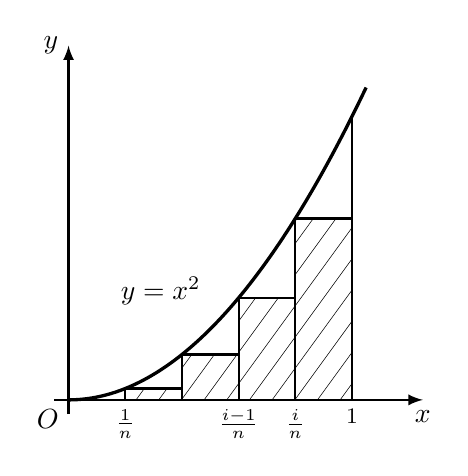
\begin{tikzpicture}[>=latex, scale=3.6]
  % 坐标轴
  \draw[->, thick] (-0.05, 0) -- (1.25, 0) node[below] {$x$};
  \draw[->, thick] (0, -0.05) -- (0, 1.25) node[left] {$y$};
  \node[below left] at (0, 0) {$O$};

  % 抛物线 y = x^2
  \draw[very thick, domain=0:1.05, smooth, samples=50] plot (\x, {\x*\x});
  \node[above left] at (0.5, 0.3) {$y=x^2$};

  % 阶梯小矩形 (示意以直代曲)
  % 矩形 i: [ (i-1)/n, i/n ], 高度 ((i-1)/n)^2
  \foreach \k/\h in {0.2/0.04, 0.4/0.16, 0.6/0.36, 0.8/0.64} {
    \draw[thick] (\k, 0) -- (\k, \h) -- (\k+0.2, \h) -- (\k+0.2, 0);
    \begin{scope}
      \clip (\k, 0) rectangle (\k+0.2, \h);
      \foreach \s in {-0.3, -0.22, ..., 1.2} {
        \draw[very thin] (\s, -0.3) -- (\s+0.8, 0.8);
      }
    \end{scope}
  }

  % x = 1 处的竖线到抛物线 (1,1)
  \draw[thick] (1, 0) -- (1, 1);

  % 轴上刻度与标注
  \node[below] at (0.2, 0) {\footnotesize $\frac{1}{n}$};
  \node[below] at (0.6, 0) {\footnotesize $\frac{i-1}{n}$};
  \node[below] at (0.8, 0) {\footnotesize $\frac{i}{n}$};
  \node[below] at (1.0, 0) {\footnotesize $1$};

  \draw (0.2, 0) -- (0.2, 0.02);
  \draw (0.4, 0) -- (0.4, 0.02);
  \draw (0.6, 0) -- (0.6, 0.02);
  \draw (0.8, 0) -- (0.8, 0.02);
  \draw (1.0, 0) -- (1.0, 0.02);
\end{tikzpicture}
\caption{}\label{fig:1.2.1}
\end{figure}

\begin{align*}
S &= \lim_{n\to+\infty}\left(\Delta S_{1}+\Delta S_{2}+\cdots+\Delta S_{n}\right) \\
&= \lim_{n\to+\infty}\frac{1}{n}\left[\left(\frac{1}{n}\right)^{2}+\left(\frac{2}{n}\right)^{2}+\cdots+\left(\frac{n-1}{n}\right)^{2}\right] \\
&= \lim_{n\to+\infty}\frac{1^{2}+2^{2}+\cdots+(n-1)^{2}}{n^{3}} = \lim_{n\to+\infty}\frac{(n-1)n(2n-1)}{6n^{3}} \\
&= \frac{1}{6}\lim_{n\to+\infty}\left(1-\frac{1}{n}\right)\left(2-\frac{1}{n}\right) = \frac{1}{3}.
\end{align*}
\end{solution}

\begin{example}\label{ex:1.2.5}
求下列极限：
\begin{enumerate}
  \item $\lim\limits_{n \to +\infty} (\sqrt{n+3} - \sqrt{n+1})$；
  \item $\lim\limits_{n \to +\infty} (\sqrt[3]{n+3} - \sqrt[3]{n+1})$；
  \item $\lim\limits_{n \to +\infty}\sqrt[n]{\lg n}$；
  \item $\lim\limits_{n\to+\infty}\sqrt[n]{a_1^n+a_2^n+\cdots+a_m^n}$（$a_i\geqslant0, i=1,2,\cdots,m$）；
  \item $\lim\limits_{n \to +\infty} [(n+1)^k - n^k]$（$0 < k < 1$）；
  \item $\lim\limits_{n \to +\infty} \left( \frac{1}{\sqrt{n^2 + 1}} + \cdots + \frac{1}{\sqrt{n^2 + n}} \right)$；
  \item $\lim\limits_{n \to +\infty} \frac{n^k}{a^n}$（$a > 1$）。
\end{enumerate}
\end{example}

\begin{solution}
(1) 因为
\[
0 < \sqrt{n+3}-\sqrt{n+1} = \frac{2}{\sqrt{n+3}+\sqrt{n+1}} < \frac{1}{\sqrt{n}} \to 0\quad (n\to+\infty),
\]
所以，由夹逼定理（或 $\varepsilon\text{-}N$ 法）知
\[
\lim_{n\to+\infty}(\sqrt{n+3}-\sqrt{n+1}) = 0.
\]

(2) 因为
\begin{align*}
0 &< \sqrt[3]{n+3}-\sqrt[3]{n+1} = \frac{2}{(\sqrt[3]{n+3})^2+\sqrt[3]{n+3}\sqrt[3]{n+1}+(\sqrt[3]{n+1})^2} \\
&< \frac{2}{3(\sqrt[3]{n})^2} = \frac{2}{3n^{\frac{2}{3}}} \to 0\quad (n\to+\infty),
\end{align*}
所以，由夹逼定理（或 $\varepsilon\text{-}N$ 法）知，
\[
\lim_{n\to+\infty}(\sqrt[3]{n+3}-\sqrt[3]{n+1}) = 0.
\]

(3) 因为
\[
10^{n} = (1+9)^{n} > 9n > n \iff 10 > n^{\frac{1}{n}} \iff 1 > \lg n^{\frac{1}{n}} = \frac{\lg n}{n} \iff \lg n < n,
\]
所以，
\[
\sqrt[n]{\lg 2} \leqslant \sqrt[n]{\lg n} < \sqrt[n]{n}.
\]
再由 $\lim\limits_{n\to+\infty}\sqrt[n]{\lg2} = 1 = \lim\limits_{n\to+\infty}\sqrt[n]{n}$ 及夹逼定理就得到
\[
\lim_{n\to+\infty}\sqrt[n]{\lg n} = 1.
\]
\textbf{注意}：虽然数列 $\{\sqrt[n]{a}\}$ 与数列 $\{\sqrt[n]{n}\}$ 的极限相同，但二者之间留有很大的空隙，这使得应用夹逼定理有极大的施展余地。

(4) 由下列不等式
\begin{align*}
\max\{a_{1},a_{2},\cdots,a_{m}\} &= \sqrt[n]{(\max\{a_{1},a_{2},\cdots,a_{m}\})^{n}} \leqslant \sqrt[n]{a_{1}^{n}+a_{2}^{n}+\cdots+a_{m}^{n}} \\
&\leqslant \sqrt[n]{n \cdot (\max\{a_{1},a_{2},\cdots,a_{m}\})^{n}} \\
&= \sqrt[n]{n}\max\{a_{1},a_{2},\cdots,a_{m}\} \to 1 \cdot \max\{a_{1},a_{2},\cdots,a_{m}\} \\
&= \max\{a_{1},a_{2},\cdots,a_{m}\}\quad (n\to+\infty)
\end{align*}
和夹逼定理知，
\[
\lim_{n\to+\infty}\sqrt[n]{a_{1}^{n}+a_{2}^{n}+\cdots+a_{m}^{n}} = \max\{a_{1},a_{2},\cdots,a_{m}\}.
\]

(5) 因为有不等式
\begin{align*}
0 < (n+1)^{k}-n^{k} &= n^{k}\left[\left(1+\frac{1}{n}\right)^{k}-1\right] < n^{k}\left[\left(1+\frac{1}{n}\right)-1\right] \\
&= \frac{1}{n^{1-k}} \to 0\quad (n\to+\infty),
\end{align*}
所以，由夹逼定理（或 $\varepsilon\text{-}N$ 法）得
\[
\lim_{n\to+\infty}[(n+1)^k-n^k] = 0.
\]

(6) 由不等式
\[
\frac{1}{1+\frac{1}{n}} < \frac{1}{\sqrt{1+\frac{1}{n}}} = \frac{n}{\sqrt{n^{2}+n}} \leqslant \frac{1}{\sqrt{n^{2}+1}}+\cdots+\frac{1}{\sqrt{n^{2}+n}} \leqslant \frac{n}{\sqrt{n^{2}+1}} < 1,
\]
$\lim\limits_{n\to+\infty}\frac{1}{1+\frac{1}{n}} = 1 = \lim\limits_{n\to+\infty}1$，以及夹逼定理立即可得
\[
\lim_{n\to+\infty}\left(\frac{1}{\sqrt{n^2+1}}+\cdots+\frac{1}{\sqrt{n^2+n}}\right) = 1.
\]

(7) 因 $a>1$，故 $\alpha = a-1 > 0$。从而
\[
0 < \frac{n^{k}}{a^{n}} = \frac{n^{k}}{(1+\alpha)^{n}} \leqslant \frac{n^{[|k|]+1}}{\mathrm{C}_{n}^{[|k|]+2}\alpha^{[|k|]+2}} \to 0\quad (n\to+\infty),
\]
再根据夹逼定理，就得 $\lim\limits_{n\to+\infty}\frac{n^k}{a^n} = 0$。
\end{solution}

\begin{example}\label{ex:1.2.6}
\begin{enumerate}
  \item 设 $a_{n} \geqslant 0$（$n \in \mathbb{N}$），$\lim\limits_{n \to +\infty} a_{n} = 0$，则 $\lim\limits_{n \to +\infty} \sqrt[n]{a_1 a_2 \cdots a_n} = 0$；
  \item 设 $a_n > 0$（$n \in \mathbb{N}$），$\lim\limits_{n \to +\infty} a_n = a > 0$，则 $\lim\limits_{n \to +\infty} \sqrt[n]{a_1 a_2 \cdots a_n} = a$。
\end{enumerate}
\end{example}

\begin{proof}
(1) 由 $0 \leqslant \sqrt[n]{a_1 a_2 \cdots a_n} \leqslant \frac{a_1 + a_2 + \cdots + a_n}{n} \to 0$（$n \to +\infty$），及夹逼定理，立即可得 $\lim\limits_{n \to +\infty} \sqrt[n]{a_1 a_2 \cdots a_n} = 0$。

(2) 当 $a>0, a_{n}>0$（$n\in\mathbb{N}$）时，有
\[
\frac{1}{\left(\frac{1}{a_{1}}+\frac{1}{a_{2}}+\cdots+\frac{1}{a_{n}}\right)/n} = \frac{n}{\frac{1}{a_{1}}+\frac{1}{a_{2}}+\cdots+\frac{1}{a_{n}}} \leqslant \sqrt[n]{a_{1}a_{2}\cdots a_{n}} \leqslant \frac{a_{1}+a_{2}+\cdots+a_{n}}{n},
\]
再由 $\lim\limits_{n\to+\infty}\frac{1}{\left(\frac{1}{a_1}+\frac{1}{a_2}+\cdots+\frac{1}{a_n}\right)/n} = \frac{1}{\frac{1}{a}} = a = \lim\limits_{n\to+\infty}\frac{a_1+a_2+\cdots+a_n}{n}$ 和夹逼定理，可得
\[
\lim_{n\to+\infty}\sqrt[n]{a_{1}a_{2}\cdots a_{n}} = a.
\]
\end{proof}

\begin{example}\label{ex:1.2.7}
设 $\lim\limits_{n\to+\infty}\sqrt[n]{|a_n|}=r>1$，则 $\lim\limits_{n\to+\infty}a_n=\infty$。
\end{example}

\begin{proof}
\textbf{证法 1} 取 $\varepsilon_{0}>0$，使得 $r-\varepsilon_{0} = 1+\alpha > 1$。因为 $\lim\limits_{n\to+\infty}\sqrt[n]{|a_{n}|} = r > 1$，故 $\exists N_{1}\in\mathbb{N}$，当 $n>N_{1}$ 时，有
\[
1+\alpha = r-\varepsilon_{0} < \sqrt[n]{|a_{n}|},\quad |a_{n}| > (1+\alpha)^{n} > n\alpha.
\]
$\forall A>0$，取 $N\in\mathbb{N}$，使得 $N > \max\left\{N_{1}, \frac{A}{\alpha}\right\}$，当 $n>N$ 时，有
\[
|a_{n}| > n\alpha > N\alpha \geqslant A.
\]
这就证明了 $\lim\limits_{n\to+\infty}a_n=\infty$。

\textbf{证法 2} 由上述，当 $n > N_{1}$ 时，有
\begin{align*}
1+\alpha &= r-\varepsilon_{0} < \sqrt[n]{|a_{n}|} < r+\varepsilon_{0} \\
&= (r-\varepsilon_{0})+2\varepsilon_{0} = 1+\alpha+2\varepsilon_{0},
\end{align*}
即 $(1+\alpha)^{n} < |a_{n}| < (1+\alpha+2\varepsilon_{0})^{n}$。所以，从 $\lim\limits_{n\to+\infty}(1+\alpha)^n = +\infty = \lim\limits_{n\to+\infty}(1+\alpha+2\varepsilon_0)^n$ 与夹逼定理可知，
\[
\lim_{n\to+\infty}|a_{n}|=+\infty \iff \lim_{n\to+\infty}a_{n}=\infty.
\]
\end{proof}

\begin{example}\label{ex:1.2.8}
设 $a_{n} \geqslant 0$（$n \in \mathbb{N}$），$\lim\limits_{n \to +\infty} \frac{a_{1} + 2a_{2} + \cdots + na_{n}}{\sqrt{n}} = a$，则
\[
\lim_{n\to+\infty}\sqrt{n} \cdot \sqrt[n]{a_{1}a_{2}\cdots a_{n}} = 0.
\]
\end{example}

\begin{proof}
\textbf{证法 1} 因为
\begin{align*}
0 &\leqslant \sqrt{n}\sqrt[n]{a_{1}a_{2}\cdots a_{n}} = \sqrt{n}\frac{\sqrt[n]{a_1 \cdot 2a_2 \cdots na_n}}{\sqrt[n]{n!}} \\
&\leqslant \frac{\sqrt{n}}{\sqrt[n]{n!}}\frac{a_{1}+2a_{2}+\cdots+na_{n}}{n} \\
&= \frac{1}{\sqrt[n]{n!}}\frac{a_{1}+2a_{2}+\cdots+na_{n}}{\sqrt{n}} \to 0 \cdot a = 0\quad (n\to+\infty),
\end{align*}
所以，根据夹逼定理，得到
\[
\lim_{n\to+\infty}\sqrt{n} \cdot \sqrt[n]{a_{1}a_{2}\cdots a_{n}} = 0.
\]

\textbf{证法 2} 由 $k(n-k+1)=(k-1)(n-k)+n \geqslant n$（$1 \leqslant k \leqslant n$）推得
\[
(n!)^{2} = (n\cdot 1)[(n-1)\cdot 2]\cdots(1\cdot n) \geqslant \underbrace{n \cdots n}_{n\text{ 个}} = n^{n}
\]
（或用数学归纳法证明）。于是，
\begin{align*}
0 &\leqslant \sqrt{n} \cdot \sqrt[n]{a_{1}a_{2}\cdots a_{n}} = \sqrt[n]{a_{1}a_{2}\cdots a_{n}n^{\frac{n}{2}}} \leqslant \sqrt[n]{a_{1}a_{2}\cdots a_{n}n!} \\
&= \sqrt[n]{a_{1}\cdot 2a_{2}\cdots na_{n}} \leqslant \frac{a_{1}+2a_{2}+\cdots+na_{n}}{n} \\
&= \frac{1}{\sqrt{n}}\frac{a_{1}+2a_{2}+\cdots+na_{n}}{\sqrt{n}} \to 0 \cdot a = 0\quad (n\to+\infty).
\end{align*}
根据夹逼定理知，$\lim\limits_{n\to+\infty}\sqrt{n}\cdot\sqrt[n]{a_1a_2\cdots a_n}=0$。
\end{proof}

\begin{exblock}{练习题 1.2}
\item 应用数列极限的基本性质求下列极限：
\begin{enumerate}
  \item $\lim\limits_{n\to+\infty}\frac{4n^2-n+5}{3n^2-2n-7}$；
  \item $\lim\limits_{n\to+\infty}\frac{3^n+(-2)^n}{3^{n+1}+(-2)^{n+1}}$；
  \item $\lim\limits_{n\to+\infty}\left(1-\frac{1}{n}\right)^{\frac{1}{n}}$；
  \item $\lim\limits_{n\to+\infty}(2\sin^{2}n+\cos^{2}n)^{\frac{1}{n}}$；
  \item $\lim\limits_{n \to +\infty} (\operatorname{arctan} n)^{\frac{1}{n}}$；
  \item $\lim\limits_{n \to +\infty} \frac{1+a+\cdots+a^{n-1}}{1+b+\cdots+b^{n-1}}$，$|a|<1, |b|<1$；
  \item $\lim\limits_{n \to +\infty} \left( \frac{1}{1 \cdot 2} + \frac{1}{2 \cdot 3} + \cdots + \frac{1}{n(n+1)} \right)$；
  \item $\lim\limits_{n \to +\infty} \left(1 - \frac{1}{2^2}\right) \left(1 - \frac{1}{3^2}\right) \cdots \left(1 - \frac{1}{n^2}\right)$；
  \item $\lim\limits_{n \to +\infty} \left( \frac{1}{2} + \frac{3}{2^2} + \cdots + \frac{2n-1}{2^n} \right)$；
  \item $\lim\limits_{n \to +\infty} \left(1 - \frac{1}{1+2}\right) \left(1 - \frac{1}{1+2+3}\right) \cdots \left(1 - \frac{1}{1+2+\cdots+n}\right)$；
  \item $\lim\limits_{n \to +\infty} \left[ \frac{1^2}{n^3} + \frac{2^2}{n^3} + \cdots + \frac{(2n-1)^2}{n^3} \right]$；
  \item $\lim\limits_{n \to +\infty} (1 + x)(1 + x^2)(1 + x^4) \cdots (1 + x^{2^{n-1}})$，其中 $|x| < 1$；
  \item $\lim\limits_{n \to +\infty} (\sqrt{n+2} - 2\sqrt{n+1} + \sqrt{n})$。
\end{enumerate}

\item 设 $a_{n} > 0, n \in \mathbb{N}$，$\lim\limits_{n \to +\infty} \frac{a_{n+1}}{a_n} = a$。应用例~\ref{ex:1.2.6} 证明：$\lim\limits_{n \to +\infty} \sqrt[n]{a_n} = a$。

\item 设 $\lim\limits_{n \to +\infty} a_n = a$。应用夹逼定理证明：$\lim\limits_{n \to +\infty} \frac{[na_n]}{n} = a$，其中 $[x]$ 表示不超过 $x$ 的最大整数。

\item 设 $a_{n} \neq 0$ 且 $\lim\limits_{n \to +\infty} \left| \frac{a_{n+1}}{a_n} \right| = r > 1$。证明：$\lim\limits_{n \to +\infty} a_{n} = \infty$。

\item 
\begin{enumerate}
  \item 应用数学归纳法或 $\frac{2k-1}{2k} < \frac{2k}{2k+1}$ 证明不等式：
  \[
  \frac{1}{2} \cdot \frac{3}{4} \cdot \cdots \cdot \frac{2n-1}{2n} < \frac{1}{\sqrt{2n+1}};
\]
  \item 证明：$\lim\limits_{n \to +\infty} \left( \frac{1}{2} \cdot \frac{3}{4} \cdot \cdots \cdot \frac{2n-1}{2n} \right) = 0$。
\end{enumerate}

\item 设 $a_n > 0$（$n \in \mathbb{N}$）且 $\lim\limits_{n \to +\infty} a_n = a > 0$。应用夹逼定理证明：$\lim\limits_{n \to +\infty} \sqrt[n]{a_n} = 1$。

\item 证明：$\lim\limits_{n \to +\infty} \frac{\sum\limits_{k=1}^{n} k!}{n!} = 1$。（提示：$1 + \frac{1}{n} \leqslant \frac{\sum\limits_{k=1}^{n} k!}{n!} \leqslant 1 + \frac{2}{n}$）。

\item 设 $\lim\limits_{n\to+\infty}a_n=a$，$\lim\limits_{n\to+\infty}b_n=b$。记
\[
S_{n}=\max\{a_{n},b_{n}\},\quad T_{n}=\min\{a_{n},b_{n}\},\quad n=1,2,\cdots.
\]
应用 $\varepsilon\text{-}N$ 法（分 $a<b, a>b, a=b$）或 $\max\{a_n, b_n\} = \frac{1}{2}(a_n + b_n + |a_n - b_n|)$ 与 $\min\{a_{n},b_{n}\}=\frac{1}{2}(a_{n}+b_{n}-|a_{n}-b_{n}|)$，证明：
\begin{enumerate}
  \item $\lim\limits_{n \to +\infty} S_n = \max\{a, b\}$；
  \item $\lim\limits_{n \to +\infty} T_n = \min\{a, b\}$。
\end{enumerate}

\item 应用例 1.1.7 与例 1.1.15 证明：
\[
\lim_{n\to+\infty}\frac{1+\sqrt{2}+\sqrt[3]{3}+\cdots+\sqrt[n]{n}}{n}=1.
\]

\item 证明：$\lim\limits_{n\to+\infty}\left(\sin\frac{\ln2}{2}+\sin\frac{\ln3}{3}+\cdots+\sin\frac{\ln n}{n}\right)^{\frac{1}{n}}=1$。

\item 证明：$\lim\limits_{n \to +\infty} \sum\limits_{k=n^{2}}^{(n+1)^{2}} \frac{1}{\sqrt{k}} = 2$。
\end{exblock}

\begin{exblock}{思考题 1.2}
\item 用 $p(n)$ 表示能整除 $n$ 的素数的个数。证明：$\lim\limits_{n\to+\infty}\frac{p(n)}{n}=0$。
\item 设 $x_{n} = \sum\limits_{k=1}^{n} \left( \sqrt{1 + \frac{k}{n^{2}}} - 1 \right)$。证明：$\lim\limits_{n \to +\infty} x_{n} = \frac{1}{4}$。
\end{exblock}
